%!TEX root = ../thesis.tex
\section{実験方法}

  実験では,学習フェーズの後にテストフェーズに移行する.以下にそれぞれの役割を示す.

  \subsubsection*{<学習フェーズ>}
  学習フェーズでは,追従対象者が再帰反射テープを装着し,\figref{Fig:RobotGuidance_course}に示す青枠で囲われた場所(ホワイエ)を2DLiDARの最大検出範囲(120\, [deg])に注意しながら,10分間ランダムに歩き回る.学習ステップ数は,0.2秒周期で学習して1stepとしているので,10分の学習で3000stepとなる.

  \subsubsection*{<テストフェーズ>}
  テストフェーズでは,2DLiDARの反射強度を利用しないため,再帰反射テープを必要としない.また,学習フェーズとは異なり,\figref{Fig:RobotGuidance_course}に示す赤枠で囲われたコースを壁に衝突せず1周できるかテストする.このコースは1周約90mであり,学習フェーズで学習したモデルを用いて,画像のみで人追従を行う.その時のロボットの挙動を確認する.

  \vspace{0.5cm}

  学習フェーズでの10分間の学習とテストフェーズでのテストコースを1周することを1セットとし,10セット実験を行った.

  \begin{figure}[h]
    \centering
    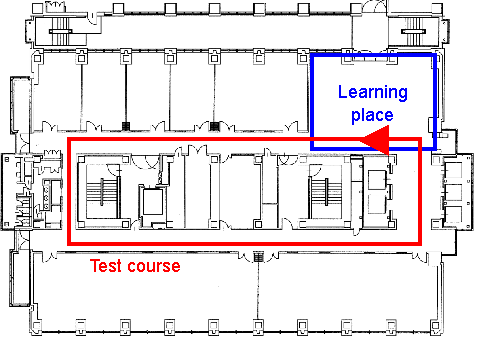
\includegraphics[width=8cm] {images/pdf/RobotGuidance_course}
    \captionsetup{justification=raggedright} % キャプションを左寄せに
    \caption{Learning and test phase courses}
    \label{Fig:RobotGuidance_course}
  \end{figure}

\newpage

\section{結果と考察}

  すべての実験でロボットが人を追従する様子が確認できた.以下にそれぞれのフェーズの様子を記述する.

  \subsubsection*{<学習フェーズ>}
  
  学習フェーズにおける実験の様子を\figref{Fig:Learning phase in experiment}に示す.2DLiDARの反射強度を入力としたルールベース制御器の出力によって,ロボットが人を追従する様子が確認できた.10セットの学習を行ったが,全てのセットにおいて人追従が継続不可能になることはなかった.

\vspace{1cm}

  \begin{figure}[h]
    \centering
    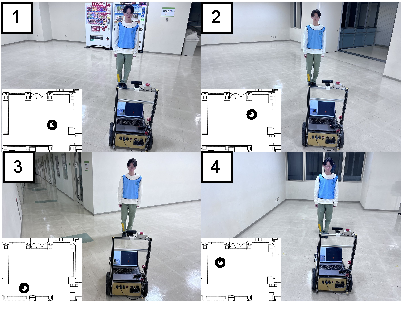
\includegraphics[width=13cm] {images/pdf/RobotGuidance_exp_learning_phase}
    \captionsetup{justification=raggedright} % キャプションを左寄せに
    \caption{Learning phase in experiment}
    \label{Fig:Learning phase in experiment}
  \end{figure}

\newpage

  \subsubsection*{<テストフェーズ>}
  
  テストフェーズにおける実験の様子を\figref{Fig:Following phase in experiment}に示す.また,それぞれの番号は以下の4つのことを表している.テストコースでは,3番に示すようにビブスに似た青色の壁紙が貼られていたが,問題なく人追従行動を継続する様子が確認できた.

  \begin{enumerate}
    \item スタート地点(ホワイエ)
    \item 1つ目の曲がり角
    \item 青色の壁紙
    \item エレベータホール
  \end{enumerate}

\vspace{1cm}

  \begin{figure}[h]
    \centering
    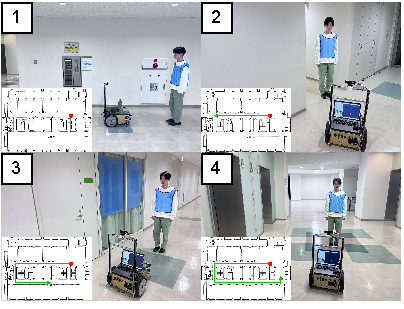
\includegraphics[width=13cm] {images/pdf/RobotGuidance_exp_test_phase}
    \captionsetup{justification=raggedright} % キャプションを左寄せに
    \caption{Test phase in experiment}
    \label{Fig:Following phase in experiment}
  \end{figure}

\newpage

  実験結果を\tabref{tab:Experiment result}に示す.10回の試行中,9回は人追従行動が継続不可能になることなく,画像を入力とした深層学習器の出力により,コースを1周することができた.一方で,10回の試行中,1回は\figref{Fig:RobotGuidance_failed_place}に示すように,テストコースの1つ目の曲がり角で壁に衝突した.ここで,学習フェーズで取得した,成功時と失敗時の角速度のヒストグラムを\figref{Fig:Histogram of angular velocity}に示す.現段階では,学習フェーズでの角速度の違いが失敗の要因と考えているが,これについてはさらなる調査が必要である.

  \begin{table}[h]
    \caption{Experiment result}
    \label{tab:Experiment result}
    \centering
    \begin{tabular}{|c|c|}
    \hline
    \hline
    Experiment & Number of success    \\ 
    \hline
    \hline
    Proposed method & 9/10 (90\%) \\ 
    \hline
    \end{tabular}
    \end{table}

  \begin{figure}[h]
    \centering
    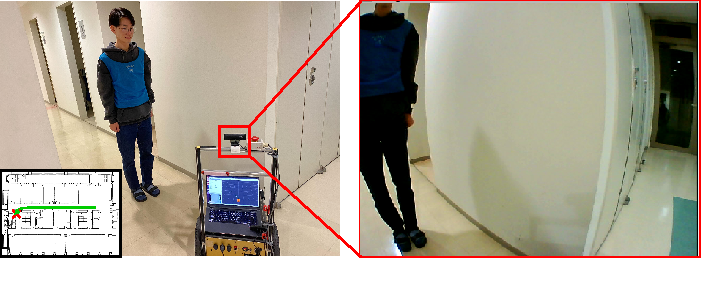
\includegraphics[keepaspectratio, scale=0.80] {images/pdf/RobotGuidance_failed_place}
    \captionsetup{justification=raggedright} % キャプションを左寄せに
    \caption{Failed at the first corner}
    \label{Fig:RobotGuidance_failed_place}
  \end{figure}

  \begin{figure}[h]
    \centering
    \begin{minipage}[c]{65mm} 
        \centering
        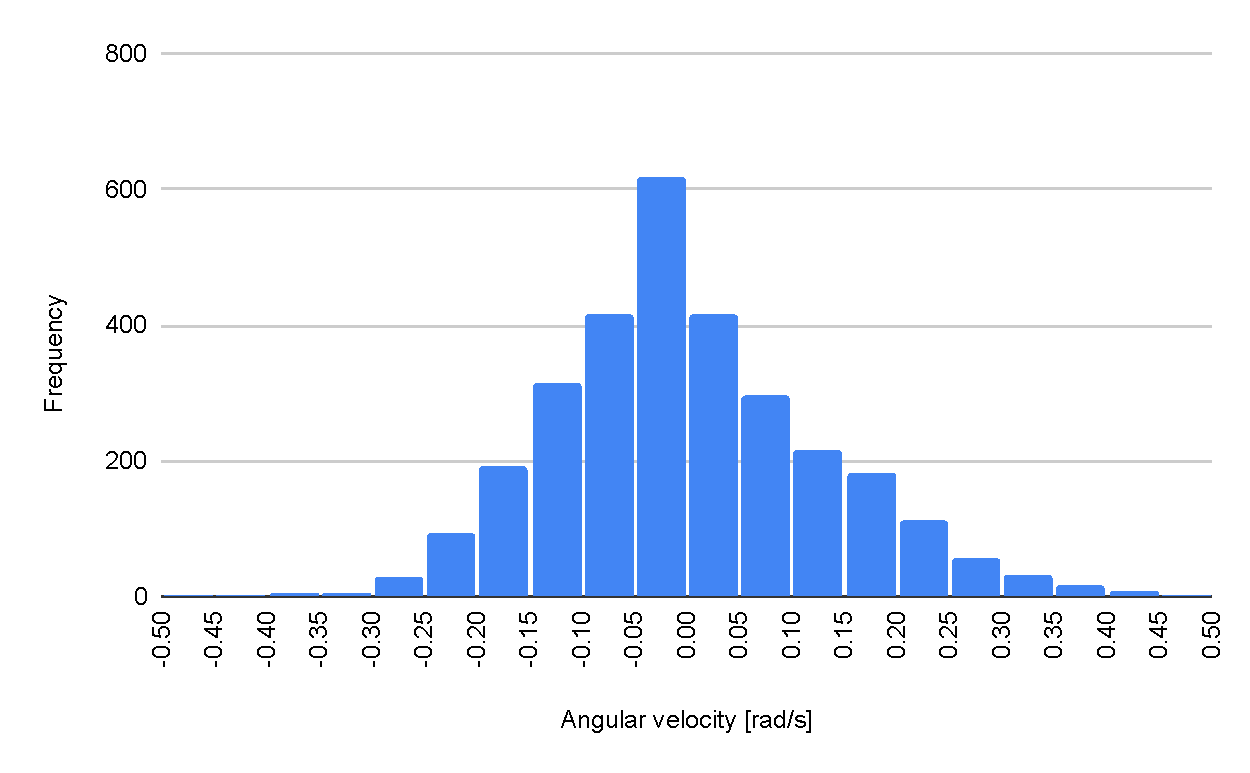
\includegraphics[height=45mm]{images/pdf/RobotGuidance_success_histogram}
        \subcaption{Success}
    \end{minipage}
    \begin{minipage}[c]{65mm} 
        \centering
        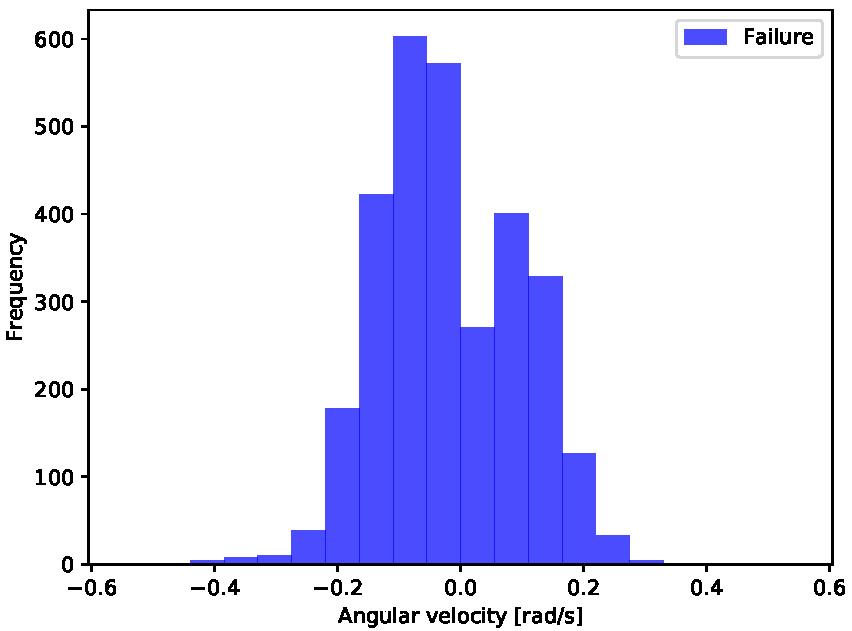
\includegraphics[height=45mm]{images/pdf/RobotGuidance_failed_histogram}
        \subcaption{Failure}
    \end{minipage}
    \caption{Histogram of angular velocity during learning phase}
    \label{Fig:Histogram of angular velocity}
  \end{figure}

\newpage
